\documentclass[12pt,a4paper]{article}
\usepackage[utf8]{inputenc}
\usepackage[catalan]{babel}
\usepackage{graphicx}
\usepackage{geometry}
\usepackage{fancyhdr}
\usepackage{tabularx}
\usepackage{lastpage}
\usepackage{enumitem}
\usepackage{amsmath}
\usepackage{tikz}

% 1. MARGES I CAPÇALERA
\geometry{top=4cm, bottom=3cm, left=2cm, right=2cm, headheight=2.5cm}

\pagestyle{fancy}
\fancyhf{}
% Assegura't de tenir els logos a la mateixa carpeta
\fancyhead[L]{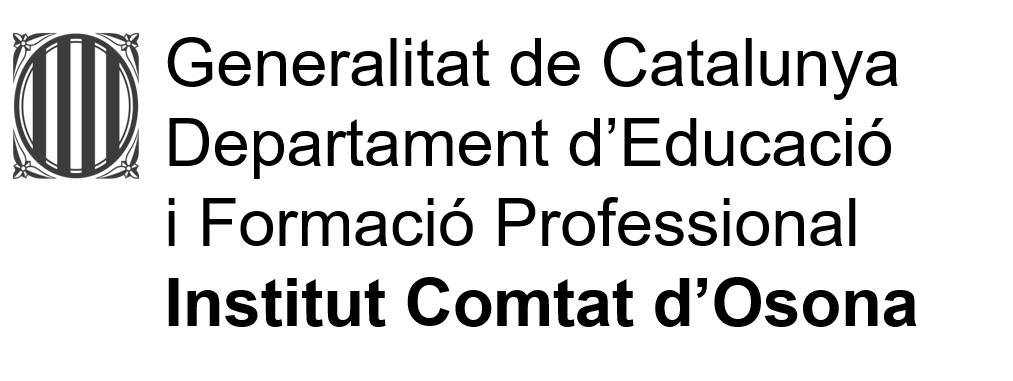
\includegraphics[height=1.8cm]{Logo_Departament.png}} 
\fancyhead[R]{
\includegraphics[height=1.8cm]{Logo_Institut.png}}

\fancyfoot[C]{Pàgina \thepage\ de \pageref{LastPage}}

\renewcommand{\headrulewidth}{0.4pt}

\begin{document}

% --- CAPÇALERA D'IDENTIFICACIÓ ---
\begingroup
\renewcommand{\arraystretch}{2.2}
\begin{tabularx}{\textwidth}{|X|p{4cm}|}
    \hline
    \textbf{Nom i cognoms:} & \textbf{Grup:} \\ \hline
    \textbf{Activitat:} Resolució de Triangles Rectangles & \textbf{Data:} \\ \hline
\end{tabularx}
\endgroup

\vspace{0.5cm}

\subsection*{Exercici 1: Trobar un angle desconegut (AS)}
A partir de les dades del triangle, identifica quins costats tens, escull la raó trigonomètrica adequada (sin, cos, tan) i calcula l'angle marcat. 

\vspace{0.5cm}

\noindent
\begin{tabularx}{\textwidth}{@{} X X @{}}
    \textbf{a)} Troba l'angle $\alpha$. & \textbf{b)} Troba l'angle $\beta$. \\[0.2cm]
    \begin{tikzpicture}[scale=0.7]
        \draw[thick] (0,0) -- (4,0) node[midway,below=3pt] {$8$} -- (0,3) -- cycle node[midway,left=2pt] {$6$};
        \draw (0.4,0) -- (0.4,0.4) -- (0,0.4); % Angle recte
        \draw (3, 0) arc (180:133.13:0.8);
        \node at (3.35,0.2) {$\alpha$};
    \end{tikzpicture} & 
    \begin{tikzpicture}[scale=0.7]
        \draw[thick] (0,0) -- (5,0) -- (0,4) node[midway,right=2pt] {$13$} -- cycle node[midway,left=2pt] {$5$};
        \draw (0.4,0) -- (0.4,0.4) -- (0,0.4); % Angle recte
        \draw (3.6,0) arc (180:118.34:0.8);
        \node at (4,0.25) {$\beta$};
    \end{tikzpicture} \\[0.5cm]
    
    \textbf{1.} Què tenim? (H, A, O?) 
    \vspace{1cm} &
    \textbf{1.} Què tenim? (H, A, O?) 
    \vspace{1cm} \\
    \textbf{2.} Quina raó trigonomètrica pots fer servir? & \textbf{2.} Quina raó trigonomètrica pots fer servir? \\[0.2cm]
    \vspace{1cm} & \vspace{1cm} \\
    
    \textbf{3.} Calcula la raó trigonomètrica: \vspace{2cm} & \textbf{3.} Calcula la raó trigonomètrica: \vspace{2cm} \\[0.2cm]
        
    \textbf{4.} Calcula l'angle: \vspace{0.5cm} & \textbf{4.} Calcula l'angle: \vspace{0.5cm}\\
    $\alpha = $  & $\beta  =$ \vspace{0.5cm}\\
\end{tabularx}
\vspace{0.2cm}

\noindent
\begin{tabularx}{\textwidth}{@{} X X @{}}
    \textbf{c)} Troba l'angle $\gamma$. & \textbf{d)} Troba l'angle $\theta$. \\[0.2cm]
    \begin{tikzpicture}[scale=0.6]
        % Dibuixem: Catet vertical -> Catet horitzontal -> Hipotenusa
        \draw[thick] (0,3.2) -- (0,0) node[midway,left=3pt] {$8$} 
                     -- (6,0) node[midway,below=3pt] {$15$} 
                     -- cycle;
        \draw (0.4,0) -- (0.4,0.4) -- (0,0.4); % Angle recte
        % Fem l'arc més gran (radi 1.2) i posem la lletra ben endins
        \draw (4.8,0) arc (180:151.93:1.2);
        \node at (4.4,0.4) {$\gamma$};
    \end{tikzpicture} & 
    \begin{tikzpicture}[scale=0.6]
        % Dibuixem: Catet vertical -> Catet horitzontal -> Hipotenusa
        \draw[thick] (0,1.75) -- (0,0) 
                     -- (6,0) node[midway,below=3pt] {$24$} 
                     -- cycle node[midway,above right=1pt] {$25$};
        \draw (0.4,0) -- (0.4,0.4) -- (0,0.4); % Angle recte
        % Fem l'arc més gran (radi 1.2) i posem la lletra ben endins
        \draw (4.8,0) arc (180:163.74:1.2);
        \node at (4.2,0.25) {$\theta$};
    \end{tikzpicture} \\
\end{tabularx}

\subsection*{Exercici 2: Trobar un costat desconegut (AS)}
A partir de l'angle i el costat que et donen, decideix quina raó trigonomètrica necessites (sin, cos, tan) per poder calcular el costat marcat amb una lletra. \textit{Aïlla bé la incògnita!}. 
\begin{itemize}
    \item \textbf{1.} Quins costats saps? Hipotenusa, Adjacent i/o Oposat?
    \item \textbf{2.} Quina raó trigonomètrica hauràs de fer servir?
    \item \textbf{3.} Planteja la fórmula i substitueix els valors coneguts.
    \item \textbf{4.} Aïlla la variable que vols correctament
\end{itemize}

\noindent
\begin{tabularx}{\textwidth}{@{} X X @{}}
    \textbf{a)} Troba el costat $x$. & \textbf{b)} Troba el costat $y$. \\
    \begin{tikzpicture}[scale=0.8]
        % Dibuixem: Catet Vertical (x) -> Catet Horitzontal -> Hipotenusa (12)
        \draw[thick] (0,2.3) -- (0,0) node[midway, left=3pt] {$x$} 
                     -- (4,0) 
                     -- cycle node[midway, above right=2pt] {$12$};
        \draw (0.3,0) -- (0.3,0.3) -- (0,0.3); % Angle recte
        \draw (3.2,0) arc (180:150:0.8);
        \node at (2.6,0.3) {$30^\circ$};
    \end{tikzpicture} & %\vspace{1cm}
    \begin{tikzpicture}[scale=0.8]
        % Dibuixem: Catet Vertical (y) -> Catet Horitzontal (7) -> Hipotenusa
        \draw[thick] (0,3) -- (0,0) node[midway, left=3pt] {$y$} 
                     -- (3,0) node[midway, below=3pt] {$7$} 
                     -- cycle;
        \draw (0.3,0) -- (0.3,0.3) -- (0,0.3); % Angle recte
        \draw (2.2,0) arc (180:135:0.8);
        \node at (1.8,0.3) {$45^\circ$};
    \end{tikzpicture} \\[3.5cm]
    
    \textbf{c)} Troba el costat $z$. & \textbf{d)} Troba el costat $w$. \\[0.2cm]
    \begin{tikzpicture}[scale=0.8]
        % Dibuixem: Catet Vertical (10) -> Catet Horitzontal (z) -> Hipotenusa
        \draw[thick] (0,4.3) -- (0,0) node[midway, left=3pt] {$10$} 
                     -- (2.5,0) node[midway, below=3pt] {$z$} 
                     -- cycle;
        \draw (0.3,0) -- (0.3,0.3) -- (0,0.3); % Angle recte
        \draw (0,3.5) arc (-90:-60:0.8);
        \node at (0.5,3.0) {$60^\circ$};
    \end{tikzpicture} & 
    \begin{tikzpicture}[scale=0.8]
        % Dibuixem: Catet Vertical -> Catet Horitzontal (8) -> Hipotenusa (w)
        \draw[thick] (0,4.7) -- (0,0) 
                     -- (4,0) node[midway, below=3pt] {$8$} 
                     -- cycle node[midway, above right=2pt] {$w$};
        \draw (0.3,0) -- (0.3,0.3) -- (0,0.3); % Angle recte
        \draw (3.2,0) arc (180:130:0.8);
        \node at (2.8,0.3) {$50^\circ$};
    \end{tikzpicture} \\[3.5cm]
\end{tabularx}
\newpage

\subsection*{Exercici 3: Resolució completa de triangles (AS)}
Resoldre un triangle significa trobar els tres costats i els tres angles. Fes els passos en ordre i deixa les operacions indicades.

\vspace{0.3cm}
\textbf{a) Se't dona un angle i la hipotenusa.} \\
\begin{minipage}{0.45\textwidth}
    \begin{tikzpicture}[scale=0.8]
        % Dibuixem: Catet vertical (b) -> Catet horitzontal (a) -> Hipotenusa (20)
        \draw[thick] (0,4.2) -- (0,0) node[midway, left=3pt] {$b$} 
                     -- (5,0) node[midway, below=3pt] {$a$} 
                     -- cycle node[midway, above right=2pt] {$20$};
        \draw (0.4,0) -- (0.4,0.4) -- (0,0.4); % Angle recte
        
        % Angle de 40 graus
        \draw (3.8,0) arc (180:140:1.2);
        \node at (4.3,0.25) {$40^\circ$};
        
        % Angle beta (a dalt)
        \draw (0,3) arc (-90:-40:1.2);
        \node at (0.6,2.5) {$\beta$};
    \end{tikzpicture}
\end{minipage}
\begin{minipage}{0.5\textwidth}
    \begin{enumerate}
        \item Recorda que els 3 angles d'un triangle sempre sumen $180^\circ$. Calcula l'angle $\beta$.
        \vspace{1cm}
        \item Troba el costat $b$ utilitzant l'angle de $40^\circ$. Si ho fas amb aquest angle, què faràs servir: cos, sin o tan? Pensa quins costats coneixes.
        \vspace{1.5cm}
        \item Troba el costat $a$ (pots utilitzar una raó trigonomètrica o un teorema que ja coneixes).
        \vspace{2cm}
    \end{enumerate}
\end{minipage}

\textbf{b) Se't donen els dos catets.} \\
\begin{minipage}{0.45\textwidth}
    \begin{tikzpicture}[scale=0.8]
        % Dibuixem: Catet vertical (9) -> Catet horitzontal (12) -> Hipotenusa (h)
        \draw[thick] (0,3) -- (0,0) node[midway, left=3pt] {$9$} 
                     -- (4,0) node[midway, below=3pt] {$12$} 
                     -- cycle node[midway, above right=2pt] {$h$};
        \draw (0.4,0) -- (0.4,0.4) -- (0,0.4); % Angle recte
        
        % Angle alfa (abaix)
        \draw (2.8,0) arc (180:143:1.2);
        \node at (3.3,0.2) {$\alpha$};
        
        % Angle beta (a dalt)
        \draw (0,1.8) arc (-90:-38:1.2);
        \node at (0.6,1.3) {$\beta$};
    \end{tikzpicture}
\end{minipage}
\begin{minipage}{0.5\textwidth}
    \begin{enumerate}
        \item Calcula la hipotenusa $h$.
        \vspace{1cm}
        \item Troba l'angle $\alpha$.
        \vspace{1.5cm}
        \item Troba l'angle $\beta$. 
        \vspace{1cm}
    \end{enumerate}
\end{minipage} \\
\newpage
\textbf{c) Se't dona la hipotenusa ($17\text{ cm}$) i un catet ($8\text{ cm}$).} \\
\textbf{Has de fer tu el dibuix del triangle rectangle}, col·locar les dades i calcular:
\begin{enumerate}
    \item El catet que falta.
    \item L'angle oposat al catet de $8\text{ cm}$.
    \item L'altre angle agut.
\end{enumerate}

\vspace{6cm}

\end{document}